\documentclass{article}
\usepackage{amsmath}
\usepackage[margin=0.5in]{geometry}
\usepackage{graphicx}
\usepackage{tikz}
\usetikzlibrary{shapes.geometric, arrows, positioning, fit, calc}


\begin{document}

\section{Forecast how tumor karyotype evolves over time in a given resource environment}

\subsection{Quantifying Chromosomal Instability (CIN)}
The next step was to translate the physical cell features from the images into a biological rate.
\begin{itemize}
    \item They developed a method to \textbf{infer chromosomal instability (CIN)} dynamics from the imaging features.
    \item Specifically, they mapped the changes in cell size, shape, and texture to the \textbf{rates of chromosome mis-segregation}—the frequency at which cells fail to divide their chromosomes correctly.
\end{itemize}

\subsection{Building the Karyotype-Transition Model (No selection)} \label{neutralModel}
With the CIN rates quantified, they built the first part of their computational model. They used the inferred chromosome mis-segregation rates to \textbf{parameterize a karyotype-transition model}. This model mathematically describes the probability of a cell's karyotype (its set of chromosomes) changing from one state to another over time due to chromosome gains and losses.

To test whether observed karyotype shifts were compatible with neutral evolution, the researchers developed a mechanistic, non-spatial agent-based simulation of karyotype evolution. The model operates as follows:

\begin{itemize}
    \item \textbf{Initialization:} Each cell lineage in the simulation is initialized with the karyotype distribution observed experimentally at the early timepoint.

    \item \textbf{Evolution:} The simulation proceeds forward for the specified number of passages, modeling cell division and potential chromosome mis-segregation events.

    \item \textbf{Core Assumptions:}
    \begin{itemize}
        \item The number of chromosome mis-segregations is proportional to the number of cell divisions, not the total elapsed time.
        \item The number of divisions per passage is assumed to be broadly comparable between different experimental conditions (e.g., control vs. starved). This implies that slower population growth is due to a longer cell-cycle duration rather than an increased rate of cell death.
        \color{blue}
        \item non-WGD cells have a close to 1 probability to die after a mis-segregations
        \color{black}
    \end{itemize}
\end{itemize}

\subsection{Modeling Hypoxia-induced Selection}
To complete the picture, they needed to model the "survival of the fittest" component driven by the low-oxygen environment.
\begin{itemize}
    \item They modeled how a cell's \textbf{oxygen demand changes based on its ploidy} (the number of chromosome sets).
    \item This allowed them to calculate the \textbf{strength of the selective pressure} exerted by hypoxia, which favors cells with ploidy levels better suited for low-oxygen survival.
\end{itemize}

\subsubsection*{Formulation of the Growth Rate Function}

At its core, the framework described in the paper comes down to formulating the growth rate of a cell as a function of its ploidy and $O_2$ availability. The model achieves this by treating the cell as an energy-based system where the rate of energy supply (dictated by $O_2$ and nutrients) must cover the costs of both survival and replication (dictated by ploidy). The energy left over after survival costs determines how quickly the cell can replicate, thus setting its growth rate.

\paragraph{Derivation of the Growth Rate Function}

\subparagraph{1. The Foundational Equation}
The model starts with the cell's energy budget, where the rate of energy supply ($U$) is balanced by the costs for survival and the costs for replication amortized over the cell cycle time ($t$):
$$
U = (U_o + U_r + U_p) + \frac{E_d + E_r + E_p}{t}
$$
Where:
\begin{itemize}
    \item $U$: Rate of energy supply to the cell.
    \item $U_o, U_r, U_p$: Ongoing energy costs for homeostasis, RNA turnover, and protein turnover (survival costs).
    \item $E_d, E_r, E_p$: Total energy costs to synthesize all DNA, RNA, and protein for a new daughter cell (replication costs).
    \item $t$: Cell cycle duration.
\end{itemize}

\subparagraph{2. Solving for Cell Cycle Time ($t$)}
To find the growth rate, we first need to determine the cell cycle time ($t$). By rearranging the equation, we can solve for $t$:
$$
t = \frac{E_d + E_r + E_p}{U - (U_o + U_r + U_p)}
$$
This shows that the time it takes to divide is the total energy needed for replication divided by the \textit{surplus} energy rate available after survival costs are met.

\subparagraph{3. Defining Growth Rate ($R$)}
Growth rate ($R$) is the inverse of the cell cycle time ($R = 1/t$). Therefore, the function for growth rate is:
$$
R = \frac{U - (U_o + U_r + U_p)}{E_d + E_r + E_p}
$$

\subparagraph{4. Incorporating Ploidy ($P$) and Oxygen ($O_2$)}
Now we express the variables as functions of ploidy and oxygen:
\begin{itemize}
    \item \textbf{Energy Supply $U(O_2)$}: The rate of energy supply, $U$, is critically dependent on oxygen availability. Under high $O_2$ (normoxia), ATP production is efficient. Under low $O_2$ (hypoxia), cells switch to less efficient glycolysis, drastically reducing $U$.
    \item \textbf{Energy Costs (functions of $P$)}: The energy costs for replication and turnover scale with the amount of cellular material, which is determined by ploidy ($P$). A tetraploid (4N) cell has roughly double the DNA, RNA, and protein of a diploid (2N) cell, and thus its energy costs are significantly higher.
    \begin{itemize}
        \item Replication Costs: $E_{total}(P) = E_d(P) + E_r(P) + E_p(P)$
        \item Survival Costs: $U_{survival}(P) = U_o + U_r(P) + U_p(P)$
    \end{itemize}
\end{itemize}


\subparagraph{5. Functional Forms of Energy Supply and Cost}
The terms $U(O_2)$, $U_{survival}(P)$, and $E_{total}(P)$ are functions, not scalars. Their forms are key to linking the cell's state and environment to its fitness.

\color{blue}
\begin{itemize}
    \item \textbf{Energy Costs ($E_{total}(P)$ and $U_{survival}(P)$):} These are best described as \textbf{linear functions of ploidy ($P$)}. The assumption is that energy requirements scale directly with cellular content. Using a diploid (P=2) cell as a baseline, the forms are:
    $$ E_{total}(P) = E_{total, 2N} \cdot \frac{P}{2} $$
    $$ U_{survival}(P) = U_o + (U_{r, 2N} + U_{p, 2N}) \cdot \frac{P}{2} $$
    Where $E_{total, 2N}$, $U_{r, 2N}$, and $U_{p, 2N}$ are the constant baseline costs for a diploid cell.

    \item \textbf{Energy Supply ($U(O_2)$):} This is a \textbf{saturating, non-linear function} of oxygen ($O_2$), resembling a Michaelis-Menten curve. This reflects the metabolic shift from efficient aerobic respiration (at high $O_2$) to inefficient glycolysis (at low $O_2$). A plausible form is:
    $$ U(O_2) = U_{min} + (U_{max} - U_{min}) \cdot \frac{O_2}{K_m + O_2} $$
    Where $U_{max}$ is the maximum energy production rate in normoxia, $U_{min}$ is the baseline rate from glycolysis in anoxia, and $K_m$ is the oxygen concentration at which the energy production rate is halfway between the minimum and maximum.
\end{itemize}
\color{black}


\begin{table}[hbt!]
\centering
\caption{\color{blue} Parameters for Model Fitting}
\label{tab:parameters}
\begin{tabular}{|c|p{5cm}|p{6cm}|}
\hline
\textbf{Parameter} & \textbf{Description} & \textbf{Role in Model Fitting} \\
\hline
$E_{total, 2N}$ & Total energy cost to replicate a baseline diploid cell. & Sets the fundamental energy barrier for cell division. \\
\hline
$(U_{r, 2N} + U_{p, 2N})$ & Rate of energy spent on RNA and protein turnover in a baseline diploid cell. & Defines the ploidy-dependent portion of the cell's "running costs". \\
\hline
$U_o$ & Rate of energy spent on basic homeostasis (ploidy-independent). & Represents the fixed survival cost that all cells must pay, regardless of size. \\
\hline
$U_{max}$ & Maximum rate of energy supply under normoxia. & Defines the upper limit of the energy budget in ideal conditions. \\
\hline
$U_{min}$ & Minimum rate of energy supply under anoxia (from glycolysis). & Defines the lower limit of the energy budget in the most severe hypoxia. \\
\hline
$K_m$ & Oxygen concentration for half-maximal energy supply. & Determines the sensitivity of the cell to hypoxia; it's the tipping point where energy supply begins to drop off sharply. \\
\hline
$\alpha_{2N}$ & Baseline lethality coefficient for diploid cells. & Defines the probability that a single segregation error is fatal in 2N cells. \\
\hline
$\beta$ & Exponent describing how tolerance scales with ploidy. & Quantifies how rapidly the lethality of mis-segregation decreases after WGD. \\
\hline
\end{tabular}
\end{table}

\subparagraph{6. The Final Function}
By substituting these dependencies, we get the final function for growth rate $R$ as a function of ploidy and oxygen:
\color{blue}
$$
R(P, O_2) = \frac{U(O_2) - U_{survival}(P)}{E_{total}(P)}
$$

This selection term will be directly plugged into section \ref{neutralModel}. \color{black} It quantitatively shows that a cell's growth rate will \textbf{decrease} if:
\begin{itemize}
    \item Oxygen ($O_2$) falls, reducing the energy supply $U(O_2)$.
    \item Ploidy ($P$) increases, raising both the survival costs $U_{survival}(P)$ and the total replication costs $E_{total}(P)$.
\end{itemize}


\subsubsection*{Fitness Implications of the Growth Rate Function}

The functional form implies that the fitness of a cell is a direct trade-off between its energy supply, dictated by the environment ($O_2$), and its energy demand, dictated by its internal state (ploidy). High ploidy cells are at an inherent energetic disadvantage due to higher costs for both survival and replication.

\paragraph{Fitness Implications: Low vs. High Ploidy}

When comparing low and high ploidy cells, the growth rate function $R(P, O_2) = \frac{U(O_2) - U_{survival}(P)}{E_{total}(P)}$ reveals two key disadvantages for high ploidy cells:

\begin{itemize}
    \item \textbf{Lower Surplus Energy}: The numerator, $U(O_2) - U_{survival}(P)$, represents the energy available for growth after basic maintenance costs are met. A high ploidy cell has greater survival costs ($U_{survival}(P)$) because it must continuously turn over a larger volume of proteins and RNA. Therefore, with the same energy supply, the high ploidy cell has less surplus energy to dedicate to proliferation.

    \item \textbf{Higher Replication Cost}: The denominator, $E_{total}(P)$, is the total energy investment required to create a new daughter cell. This cost is substantially higher for high ploidy cells as they must synthesize much more DNA, RNA, and protein to duplicate themselves. This means that even with the same amount of surplus energy, a high ploidy cell takes longer to accumulate the resources needed to divide.
\end{itemize}

Essentially, high ploidy cells have higher "overhead" and a larger "capital investment" for each division, making their growth rate acutely sensitive to the available energy supply.

\paragraph{Fitness under High Oxygen Concentrations}

Under high oxygen concentrations (normoxia), the energy supply, $U(O_2)$, is abundant. In this scenario, the model predicts that the fitness difference between low and high ploidy cells is minimal.

When $U(O_2)$ is very large, there is more than enough energy to cover the elevated survival ($U_{survival}(P)$) and replication ($E_{total}(P)$) costs of the high ploidy cells. The abundance of energy effectively masks the inherent inefficiency of the high ploidy state. The paper supports this by noting that experiments showing no negative effects of aneuploidy were conducted in resource-rich conditions and that the selection coefficient against polyploid cells is expected to be zero when energy is not a limiting factor. Therefore, in a high-oxygen environment, high ploidy cells can proliferate at rates nearly comparable to their low ploidy counterparts.



\subsection{Modeling Post-Missegregation Death as a Function of WGD Status}
To complete the model of fitness under genomic instability, we next consider how cells survive or die following chromosome mis-segregation (MS) events. The probability that a cell survives an MS event depends on its genomic architecture—particularly whether it has undergone whole-genome duplication (WGD). Diploid cells (2N) are less tolerant of chromosome losses or gains because each mis-segregation affects a larger fraction of the genome, while tetraploid (4N) cells, with duplicated genetic content, can buffer such perturbations.

\begin{itemize}
    \item We define a \textbf{mis-segregation tolerance function} that captures how WGD status modifies the likelihood of survival after an MS event.
    \item This function links the cell’s \textbf{chromosomal instability rate (CIN)}—the probability of a segregation error per chromosome per division—to the \textbf{probability of cell death ($D_{MS}$)} that follows such an event.
\end{itemize}

\subsubsection*{Formulation of the Death Probability Function}

Let $\mu$ denote the per-chromosome mis-segregation rate and $n(P)$ the number of chromosome copies at ploidy $P$. For a given division, the expected number of segregation errors is $\mu \cdot n(P)$. Not every error is lethal: the probability of death depends on both the number of errors and the cell’s tolerance.

\paragraph{1. Base Model for Death Probability}
We define the survival probability after an MS event as:
\[
S_{MS}(P) = \exp[-\alpha(P) \cdot \mu \cdot n(P)],
\]
where $\alpha(P)$ is the \textbf{MS sensitivity coefficient}—a parameter describing how damaging a single segregation error is at ploidy $P$.

The probability of death is then:
\[
D_{MS}(P) = 1 - S_{MS}(P) = 1 - \exp[-\alpha(P) \cdot \mu \cdot n(P)].
\]

\paragraph{2. Dependence on WGD Status}
\color{blue} To model the protective effect of WGD, we define:
\[
\alpha(P) = \alpha_{2N} \cdot \left(\frac{2}{P}\right)^{\beta},
\]
where $\alpha_{2N}$ is the baseline lethality coefficient for diploid cells and $\beta$ is an empirical exponent capturing how rapidly tolerance increases with ploidy. \color{black} For example, $\beta \approx 1$ implies that doubling the genome content halves the impact of a segregation error.

Thus, for 4N cells:
\[
D_{MS}(4N) = 1 - \exp[-\alpha_{2N} \cdot \left(\frac{1}{2}\right)^{\beta} \cdot \mu \cdot n(4N)].
\]
This relation ensures that WGD cells exhibit a lower probability of immediate death following mis-segregation, consistent with experimental observations of their enhanced tolerance to aneuploidy (Table \ref{tab:parameters}).




\subsection{Explaining an Unexpected Observation}
Finally, they addressed a surprising result from their 2N experiments.

They observed that in the 2N populations, there was an initial, rapid expansion of newly formed 4N cells, which seemed counterintuitive since selection later favored lower ploidy.

They explained this by either:
\color{blue}
\begin{itemize}
    \item identifying a transient nutritional advantage where the new 4N cells gained resources by engaging in cannibalistic interactions with the surrounding 2N cells.
    \item the tolerance of WGD cells to hypoxia induced increases in CIN
\end{itemize}
\color{black}

\subsection{Integrating and Validating the Final Framework}
\color{blue}
 They validated this comprehensive framework by showing it could accurately \textbf{reproduce the ploidy reduction} they observed in their 4N cell experiments as well as the \textbf{WGD} observed in the 2N cells, and could also \textbf{forecast evolutionary trajectories} under different simulated oxygen conditions.
\color{black}



\section{Modeling drug-induced selection }
The same framework can be adapted to model selection driven by a therapeutic agent. This approach is more phenomenological, relying on fitting standard dose-response curves where the parameters of the curve are themselves functions of ploidy.

\subsubsection*{Formulation of the Growth Rate Function R(P, D)}

The growth rate $R$ at a given drug dose $D$ can be described by a standard Hill function, which creates a sigmoidal dose-response curve. To account for ploidy, we make the parameters of this curve dependent on ploidy ($P$):
\begin{itemize}
    \item \textbf{$R_{max}(P, O_2)$:} The maximum growth rate in the absence of the drug (D=0). This is simply the baseline growth rate from the previous model, $R(P, O_2)$.
    \item \textbf{$EC50(P)$:} The drug concentration that produces 50\% inhibition. This parameter measures drug potency. If high-ploidy cells are more sensitive to a drug, their $EC50$ will be lower, meaning $EC50(P)$ is a decreasing function of $P$.
    \item \textbf{$h(P)$:} The Hill slope, describing the steepness of the response. This may also vary with ploidy.
\end{itemize}

By substituting these ploidy-dependent parameters, we get the final function:
\color{blue}
$$
R(P, D) = R_{max}(P, O_2) \cdot \left(1 - \frac{D^{h(P)}}{EC50(P)^{h(P)} + D^{h(P)}}\right)
$$
\color{black}

\subsubsection*{Functional Forms for Ploidy-Dependent Parameters}
To make the model flexible, we can define $EC50(P)$ and $h(P)$ using simple functional forms that can capture either an increase or decrease in drug response with ploidy. Linear functions are a straightforward choice:

\begin{itemize}
    \item \textbf{EC50 as a function of Ploidy ($EC50(P)$):} We can model the change in drug potency with a linear relationship, centered around the diploid (P=2) state:
    $$ EC50(P) = EC50_{2N} + \beta \cdot (P - 2) $$
    \color{blue}
    The parameter $\beta$ determines the relationship. If $\beta < 0$, higher ploidy leads to a lower EC50 (increased sensitivity: \textbf{ high-ploidy treatment regime}). If $\beta > 0$, higher ploidy leads to a higher EC50 (increased resistance:  \textbf{low-ploidy treatment regime}).
    \color{black}
    \item \textbf{Hill Slope as a function of Ploidy ($h(P)$):} Similarly, the Hill slope can be modeled as a linear function:
    $$ h(P) = h_{2N} + \gamma \cdot (P - 2) $$
    \color{blue}
    The parameter $\gamma$ determines how the steepness of the dose-response curve changes with ploidy.
    \color{black}
\end{itemize}

\begin{figure}[h!]
\centering
\framebox{\parbox{0.6\textwidth}{\centering
\vspace{4cm}
\textbf{Image Placeholder} \\
\small\textit{Two dose-response curves showing a lower EC50 for high-ploidy cells (more sensitive) compared to low-ploidy cells.}
\vspace{4cm}
}}
\caption{Ploidy-dependent drug response curves. The increased sensitivity of high-ploidy cells is captured by a left-shift in the curve (lower EC50).}
\label{fig:drug_response}
\end{figure}

\subsubsection*{Parameters for Model Fitting}
To fit this model to experimental data, the key parameters from the dose-response curves would need to be determined for different ploidy levels.

\begin{table}[h!]
\centering
\caption{\color{blue} Parameters for Drug-Response Model Fitting \color{black}}
\label{tab:drug_parameters}
\begin{tabular}{|c|p{5cm}|p{6cm}|}
\hline
\textbf{Parameter} & \textbf{Description} & \textbf{Role in Model Fitting} \\
\hline
$EC50_{2N}$ & The EC50 value for baseline diploid (P=2) cells. & Anchors the drug potency measurement. \\
\hline
$h_{2N}$ & The Hill slope for baseline diploid (P=2) cells. & Anchors the drug response steepness. \\
\hline
$\beta$ & The coefficient determining the change in EC50 with ploidy. & Models whether drug sensitivity increases ($\beta < 0$) or decreases ($\beta > 0$) with ploidy. \\
\hline
$\gamma$ & The coefficient determining the change in the Hill slope with ploidy. & Models how the cooperativity of the drug response changes with ploidy. \\
\hline
\label{drugresponse}
\end{tabular}
\end{table}


\section{Modeling Adaptive Drug Sequencing}
With a complete model of ploidy evolution under drug selection, we can design an algorithm for an adaptive therapeutic strategy. The goal is to dynamically select or switch drugs to maximally suppress tumor growth by exploiting the evolving ploidy composition of the cell population.


   % \item Select a treatment regime: either High-Ploidy (HP) targeting (drugs with $\beta < 0$) or Low-Ploidy (LP) targeting (drugs with $\beta > 0$) depending on the tumor's dominant ploidy state.

  
\subsection{Identify the optimal sequence of drugs within each ploidy-specific regime}

To bridge the gap between the pre-clinical model and clinical reality, we propose a hybrid algorithm that uses observed patient response data to continuously correct and personalize the predictive model. This approach accounts for ploidy-independent, patient-to-patient variability in drug response.

\subsubsection*{Introducing a Patient-Specific Efficacy Parameter}
We introduce a patient-specific efficacy parameter, $\alpha_i$, for each drug $i$. This parameter acts as a scaling factor on the drug's effect, capturing individual variability beyond what is explained by ploidy alone. The growth rate function is modified to include this parameter:
$$
R(P, D, drug_i) = R_{max}(P) \cdot \left(1 - \alpha_i \cdot \frac{D^{h(P)}}{EC50(P)^{h(P)} + D^{h(P)}}\right)
$$
\color{blue}, where D is the clinical drug dose \color{black}. Initially, we assume $\alpha_i = 1$ for all drugs, meaning our first prediction relies solely on the general, ploidy-based model. This parameter is then updated based on clinical observation.

\subsubsection*{Algorithm for Adaptive Therapy with Efficacy Correction}
The algorithm iterates through cycles of prediction, treatment, observation, and model calibration, relying on a simulated ploidy distribution when direct measurements are unavailable.

\begin{enumerate}
    \item \textbf{Initial Drug Selection (at $t=0$):}
    \begin{itemize}
        \item Measure the initial tumor ploidy distribution, $f(P, t=0)$.
        \item For each drug $i$, calculate the predicted mean growth rate assuming baseline efficacy ($\alpha_i=1$):
        $$ \bar{R}_{predicted, i}(t=0) = \sum_{P} f(P, t=0) \cdot R(P, D, drug_i, \alpha_i=1) $$
        \item Select the drug that minimizes this predicted growth rate. Let this be Drug A.
    \end{itemize}
    
    \item \textbf{Treat and Observe (Interval $\Delta t$):}
    \begin{itemize}
        \item Administer Drug A for a time interval $\Delta t$.
        \item At the end of the interval, measure the \textit{observed} mean growth rate of the tumor, $\bar{R}_{observed, A}$, based on the change in tumor burden.
    \end{itemize}

    \item \textbf{Model Correction (Efficacy Parameter Updating):}
    \begin{itemize}
        \item Compare the model's initial prediction, $\bar{R}_{predicted, A}(t=0)$, with the observed outcome, $\bar{R}_{observed, A}$.
        \item Solve for the patient-specific efficacy parameter, $\alpha'_A$, that makes the model match the observation. This is done by solving the following equation for $\alpha'_A$:
        $$ \bar{R}_{observed, A} = \sum_{P} f(P, t=0) \cdot R(P, D, \text{Drug A}, \alpha'_A) $$
        \item \color{blue} This step calibrates the model for Drug A, capturing its true efficacy in this patient. The parameter $\alpha'_A$ now represents a learned, patient-specific correction factor \color{black}.
    \end{itemize}

    \item \textbf{Re-assessment and Switching Decision (at $t+\Delta t$):}
    \begin{itemize}
        \item \textbf{Simulate Ploidy Evolution:} \color{blue} Generate a \textit{predicted} ploidy distribution for the next time point, $f_{predicted}(P, t+\Delta t)$. This is done by simulating the tumor's evolution over the interval $\Delta t$ starting from the last known distribution, $f(P, t)$, under the selective pressure of Drug A with its newly calibrated efficacy parameter $\alpha'_A$.
        \item \textbf{Project Future Efficacy:} Using this predicted ploidy distribution, $f_{predicted}(P, t+\Delta t)$, project the mean growth rate for \textit{all} available drugs. \color{black}
        \item For Drug A, use its \textbf{updated} efficacy parameter $\alpha'_A$.
        \item For all other drugs $j \neq A$, for which we have no direct data yet, continue to use the baseline efficacy $\alpha_j=1$.
        $$ \bar{R}_{projected, i}(t+\Delta t) = \sum_{P} f_{predicted}(P, t+\Delta t) \cdot R(P, D, drug_i, \alpha'_i) $$
        (where $\alpha'_i = \alpha'_A$ if $i=A$, and $\alpha'_i = 1$ otherwise)
        \item Identify the drug that now yields the minimum projected mean growth rate. Let this be Drug B.
        \item \textbf{Switching Rule:} If Drug B is different from Drug A, switch the treatment to Drug B. Otherwise, continue with the now-calibrated Drug A.
    \end{itemize}
    
    \item \textbf{Iteration:}
    \begin{itemize}
        \item Repeat Steps 2 through 4. The predicted ploidy distribution from the end of one cycle, $f_{predicted}(P, t+\Delta t)$, becomes the starting distribution for the simulation in the next cycle. Each time a drug is used, its $\alpha$ parameter is calibrated, making the model's predictions progressively more accurate.
    \end{itemize}
\end{enumerate}

%%@TODO: predicted ploidy distribution switch to low ploidy --> trigger biopsy. alhorithm for switch between low- vs. high ploidy


\subsection{Determine when to transition between low- and high-ploidy treatment regimes}


\textbf{Triggering a New Ploidy Quantification (Risk Assessment):}
    At the end of each cycle, before committing to the next treatment interval, the algorithm assesses whether a new ploidy measurement is warranted. A new biopsy is recommended if one of two conditions is met:
    \begin{itemize}
        \item \textbf{Condition 1: Model Uncertainty Exceeds Threshold.} The model's cumulative uncertainty is quantified using a \textbf{Risk Score}.
        \begin{itemize}
            \item \textbf{Divergence Score ($S_{divergence}$):} \color{blue} This measures how "surprising" the most recent clinical observation was. A large discrepancy between the predicted growth rate under the \textbf{un}calibrated model and the observed growth rate suggests the underlying ploidy simulation may be wrong (e.g. because a WGD event happened or a rare, pre-existing WGD- clone expanded or error propagation over time).
            $$ S_{divergence} = |\bar{R}_{observed, A} - \bar{R}_{projected, A}(t+\Delta t)| $$
            \color{black} 
            \item \textbf{Time Penalty ($P_{time}$):} This score increases with the time elapsed since the last biopsy, $\Delta t_{biopsy}$, reflecting the accumulating uncertainty from unobserved CIN.
            $$ P_{time} = 1 + k \cdot \Delta t_{biopsy} $$
            Here, $k$ is a constant representing the rate of uncertainty accumulation.
            \item \textbf{Combined Risk Score:} The total risk is a product of these two factors.
            $$ \text{Risk Score} = S_{divergence} \cdot P_{time} $$
        \end{itemize}

        \item \textbf{Condition 2: Predicted Shift in Ploidy Regime.} \color{blue} A biopsy is also triggered to confirm the model's state before making a high-stakes change in therapeutic strategy (i.e., switching between a drug targeting high-ploidy cells and one targeting low-ploidy cells). \color{black} 
        \begin{itemize}
            \item Let Drug A be the current drug and Drug B be the new optimal drug predicted in Step 4.
            \item Let $\beta_A$ and $\beta_B$ be their respective ploidy-sensitivity parameters.
            \item A regime shift is predicted if the drugs target opposite ends of the ploidy spectrum. This occurs if:
            $$ \text{sign}(\beta_A) \neq \text{sign}(\beta_B) \quad  $$
        \end{itemize}

        \item \textbf{Triggering Rule:}
        $$ \text{If (Risk Score} > \theta) \lor (\text{Regime Shift Predicted}) \rightarrow \text{Recommend New Biopsy} $$
        Upon receiving new ploidy data, the algorithm resets $\Delta t_{biopsy}$ to zero and uses the new $f(P,t)$ as the starting point for the next cycle.
    \end{itemize}
    
    
    \begin{itemize}
        \item Repeat Steps 2 through 5. The predicted ploidy distribution from the end of one cycle, $f_{predicted}(P, t+\Delta t)$, becomes the starting distribution for the simulation in the next cycle. Each time a drug is used, its $\alpha$ parameter is calibrated, making the model's predictions progressively more accurate.
    \end{itemize}


\begin{table}[h!]
\centering
\caption{\color{blue} Parameters for Risk Assessment}
\label{tab:risk_parameters}
\begin{tabular}{|c|p{5cm}|p{6cm}|}
\hline
\textbf{Parameter} & \textbf{Description} & \textbf{Role in Model Fitting} \\
\hline
$k$ & Rate of uncertainty accumulation. & A hyperparameter that scales how quickly the model's confidence decays over time without new ploidy data. Could be estimated from CIN rates. \\
\hline
$\theta$ & Clinical risk threshold. & A pre-defined value set by clinicians that represents the maximum acceptable level of model uncertainty before a new measurement is deemed necessary. \\
\hline
\end{tabular}
\end{table}



\begin{figure}[h!]
\centering
\resizebox{\textwidth}{!}{%
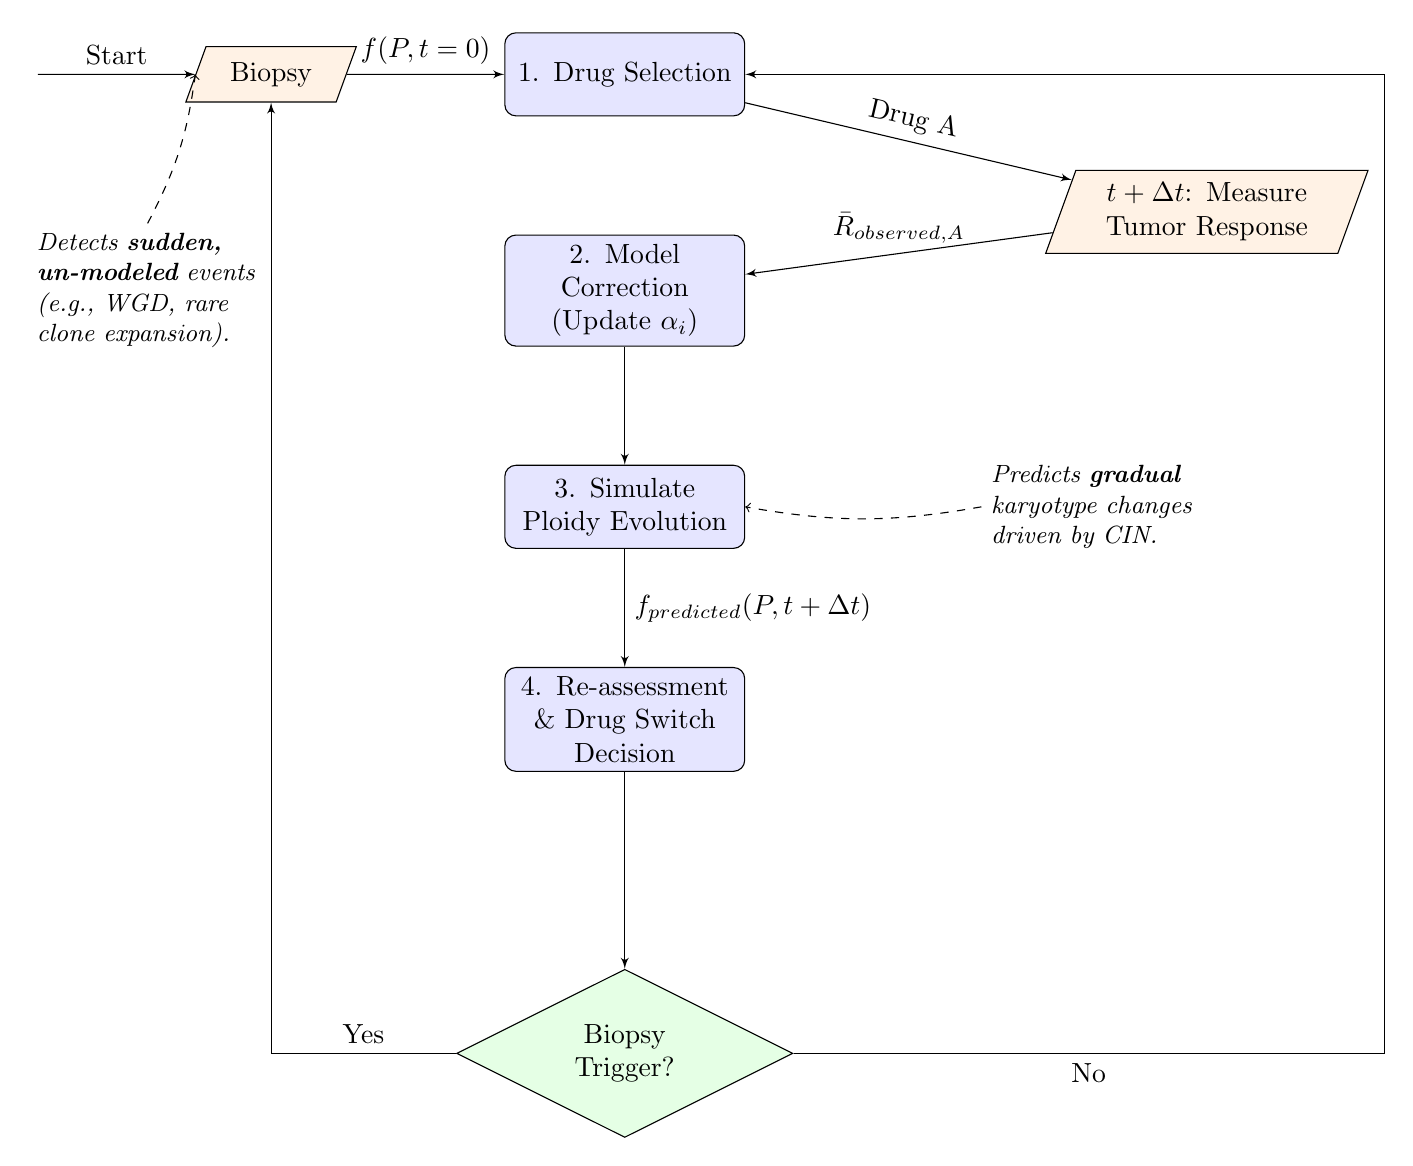
\begin{tikzpicture}[
    node distance=1.5cm and 2cm,
    block/.style={rectangle, draw, fill=blue!10, text width=8em, text centered, rounded corners, minimum height=3em},
    line/.style={draw, -latex'},
    cloud/.style={ellipse, draw, fill=red!10, minimum height=2em, text width=7em, text centered},
    decision/.style={diamond, draw, fill=green!10, text width=6em, text centered, aspect=2},
    io/.style={trapezium, trapezium left angle=70, trapezium right angle=110, draw, fill=orange!10, text centered, minimum height=2em},
    iob/.style={trapezium, trapezium left angle=70, trapezium right angle=110, draw, fill=orange!10, text width=8em, text centered, minimum height=3em},
    note/.style={rectangle, text width=8em, align=left, font=\small\itshape}
]

% Nodes for Clinical Reality
\node[io] (biopsy) {Biopsy};

% Nodes for Computational Model
\node[block, right=of biopsy] (initial_drug) {1. Drug Selection};
\node[block, below=of initial_drug] (model_correction) {2. Model Correction (Update $\alpha_i$)};
\node[block, below=of model_correction] (simulate_ploidy) {3. Simulate Ploidy Evolution};
\node[block, below=of simulate_ploidy] (reassess) {4. Re-assessment \& Drug Switch Decision};
\node[decision, below=of reassess, yshift=-1cm] (biopsy_trigger) {Biopsy Trigger?};

% Move 'Measure Tumor Response' to be slightly above and to the right of 'Model Correction'
\node[iob, right=of model_correction, xshift=2cm, yshift=1cm] (measure_response) {$t+\Delta t$:  Measure Tumor Response};

% Main flow
\node[coordinate, left=of biopsy] (start) {};
\path [line] (start) -- node[above] {Start} (biopsy);
\path [line] (biopsy) -- node[above] {$f(P, t=0)$} (initial_drug);
\path [line] (initial_drug) -- node[above, sloped] {Drug A} (measure_response);
\path [line] (measure_response) -- node[above] {$\bar{R}_{observed, A}$} (model_correction);
\path [line] (model_correction) -- (simulate_ploidy);
\path [line] (simulate_ploidy) -- node[right] {$f_{predicted}(P, t+\Delta t)$} (reassess);
\path [line] (reassess) -- (biopsy_trigger);
% Corrected Path: Go right, then use |- to go up and left to the target.
\path[line] (biopsy_trigger.east) -- ++(7.5,0) node[midway, below]{No} |- (initial_drug.east);
\path [line] (biopsy_trigger.west) -| node[pos=0.25, above] {Yes} (biopsy);

% Explanatory Notes
\node[note, right=of simulate_ploidy, xshift=1cm] (note_cin) {Predicts \textbf{gradual} karyotype changes driven by CIN.};
\path[draw,->,dashed] (note_cin.west) to [bend left=10] (simulate_ploidy.east);

\node[note, left=of model_correction, xshift=-1cm] (note_wgd) {Detects \textbf{sudden, un-modeled} events (e.g., WGD, rare clone expansion).};
\path[draw,->,dashed] (note_wgd.north) to [bend right=10] (biopsy.west);

\end{tikzpicture}
}
\caption{Diagram of the Adaptive/Extinction Therapy Decision Framework. The framework integrates clinical measurements with a computational model to create a feedback loop. The model predicts gradual ploidy evolution, while discrepancies between its predictions and observed tumor responses allow it to detect and adapt to sudden, un-modeled events, triggering a new biopsy when uncertainty becomes too high. \color{blue} We can switch between drugs \textbf{within} a regime based on model predictions + tumor response alone, but we require biopsy to switch \textbf{between} regimes.}
\label{fig:framework_diagram}
\end{figure}

\end{document}

% interplay between the clinical world (measurements) and the computational model (predictions). It highlights how the karyotype evolution model predicts gradual changes, while the integration of observed tumor response allows the system to detect and react to un-modeled, sudden events like Whole-Genome Doubling.